\begin{figure*}[!htb] % concept
  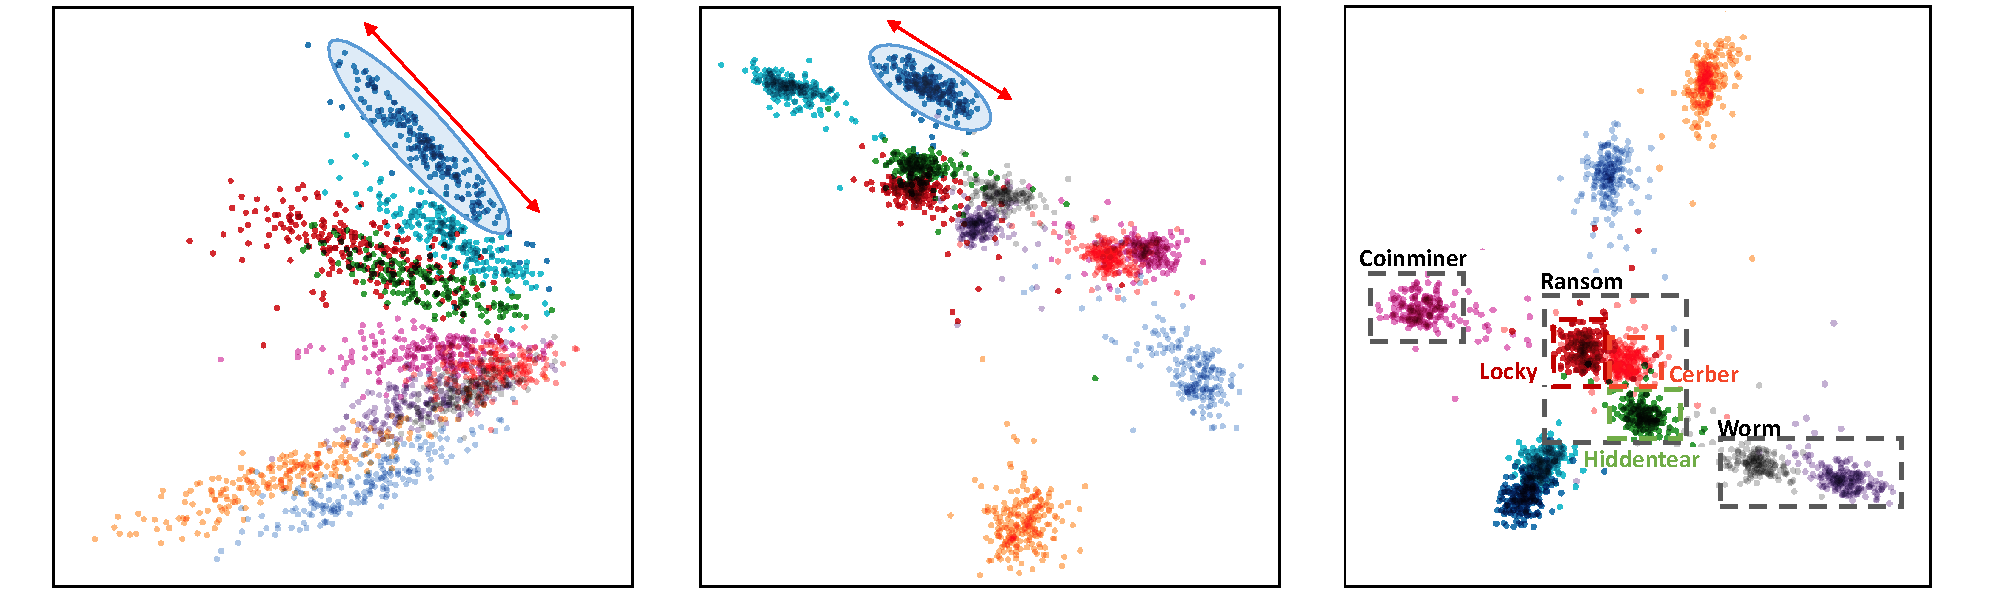
\includegraphics[width=\textwidth]{../../figures/concept.pdf}
  \caption{concept}
  \label{fig:concept}
\end{figure*}

\section{Semantics Aware Representation Learning}
이번 섹션에서는 Auxiliary task 를 통해 malware를 멀웨어 시멘틱 스페이스 위에서 해석할 수 있게 임베딩시키는 방법을 설명한다. 먼저 우리가 정의한 멀웨어 시멘틱 스페이스가 무엇인지 설명하고, semantic-aware malware representation vector 를 학습하기 위한 Loss function 을 제안한다.

\subsection{Semantic Spaces for Malwares}

\textbf{Definition. }
Let $X = \{x_1, …, x_n, …, x_N\}$ be a set of malwares.
Let $S$ be a subset of vector space $V$ of dimension $d$ and let semantic component set $S = \{s_1, ... , s_k, … s_K\}$ be a linearly independent subset of $V$.  
Then for every $\mathbf{e} \in E$, there is an unique linear combination of the sementic component vectors that equals $e$.
\[
\mathbf{e} = c_1\mathbf{s_1} + c_2\mathbf{s_2} + … + c_k\mathbf{s_k} 
\]

where $c_i$ is the i’th element of coefficient vector $ \mathbf{c} = \{c_1, ... , c_k\}$
We call a vector $e$ as a semantic vector of malware $x$ and there is a nonlinear mapping from $X$ to $E$. 

\textbf{Metric function. }
we use an Euclidean Distance $d(e_i, e_j)$ for a metric of a set E and it means the function that defines a distance between  semantics of two malwares. 

\textbf{The meaning of a learning malware semantic space. }
Malware semantic space 를 배운다는 것은 무슨 뜻일까.
언어를 예를 들어보자. 우리는 머릿속으로 어떤 단어들의 의미을 생각해볼 수 있다. 그 의미들의 관계를 생각해보자. 도시 이름들과 머신 러닝에 관련된 단어들은 멀리 위치한다고 생각해볼 수 있다. 그리고 각각은 가까울 것이라고 생각할 수 있다. 단어들 간 관계의 유사성을 생각해볼 수 도 있다. King 과 Queen 의 관계는 Man 과 Woman 의 관계와 비슷하다는 생각을 해볼 수 있다. 이렇게 머릿 속에 존재하는 단어들의 의미를 최대한 approximate 해서 표현하려면, 벡터 스페이스 위에 개념들을 벡터로서 올려보는 방법이 있다. 의미가 가깝다면 벡터 간 거리가 가깝게,  의미가 멀다면 벡터 간 거리가 멀게 위치시킬 수 있다. king - queen = man - woman 와 같이, 벡터스페이스에서 정의된 연산을 이용해서 우리가 머릿속으로 생각하는 단어들 간의 관계를 모사(approximate)하여 표현해볼 수도 있다. 

마찬가지로 우리는 머릿속에서 악성코드의 의미를 생각해볼 수 있다. 우리는 악성코드가 악성 컴포넌트들의 조합이라고 여기고, 이를 벡터 스페이스의 연산으로 모사(approximate)하여 표현하기 위해, basis 와 Linear combination 이라는 개념을 이용하였다. 즉, 멀웨어의 sematnic vector 가 semantic component vector의 선형 조합으로 표현되도록 가르치는 것은 우리의 머릿 속에 존재하는 Semantics 를 벡터 스페이스에서 최대한 따라하겠다는 것이고 이것의 의미가 바로 Semantic space 를 학습한다는 의미이다. 

\textbf{Evidences. } 우리가 위에서 정의한대로 Semantic space를 잘 학습했다면 다음 쿼링 태스크들이 제대로 작동해야한다. 먼저 멀웨어 샘플로 쿼링해서 의미가 비슷한 샘플들을 검색할 수 있어야 한다. 둘째로, semantic components의 조합 만으로 검색할 수 있어야 한다. 이를테면, ransom, downloader, agent 세 가지 속성을 모두 갖는 멀웨어를 검색할 수 있어야한다. 마지막으로, 샘플과 semantic components 의 조합으로 검색할 수 있어야 한다. 이를테면, ransom, downloader 의 속성을 갖는 샘플과 agent 라는 semantic component 를 함께 검색하여 세 속성 모두 갖는 샘플들을 검색할 수 있어야 한다. 이 쿼리 방법들에 대한 그림 설명은 Figure.\ref{fig:qualitative_all} 에서 확인할 수 있다. 

\subsection{Solution Overview}
\begin{figure*}[!htb] % qualitative_all
  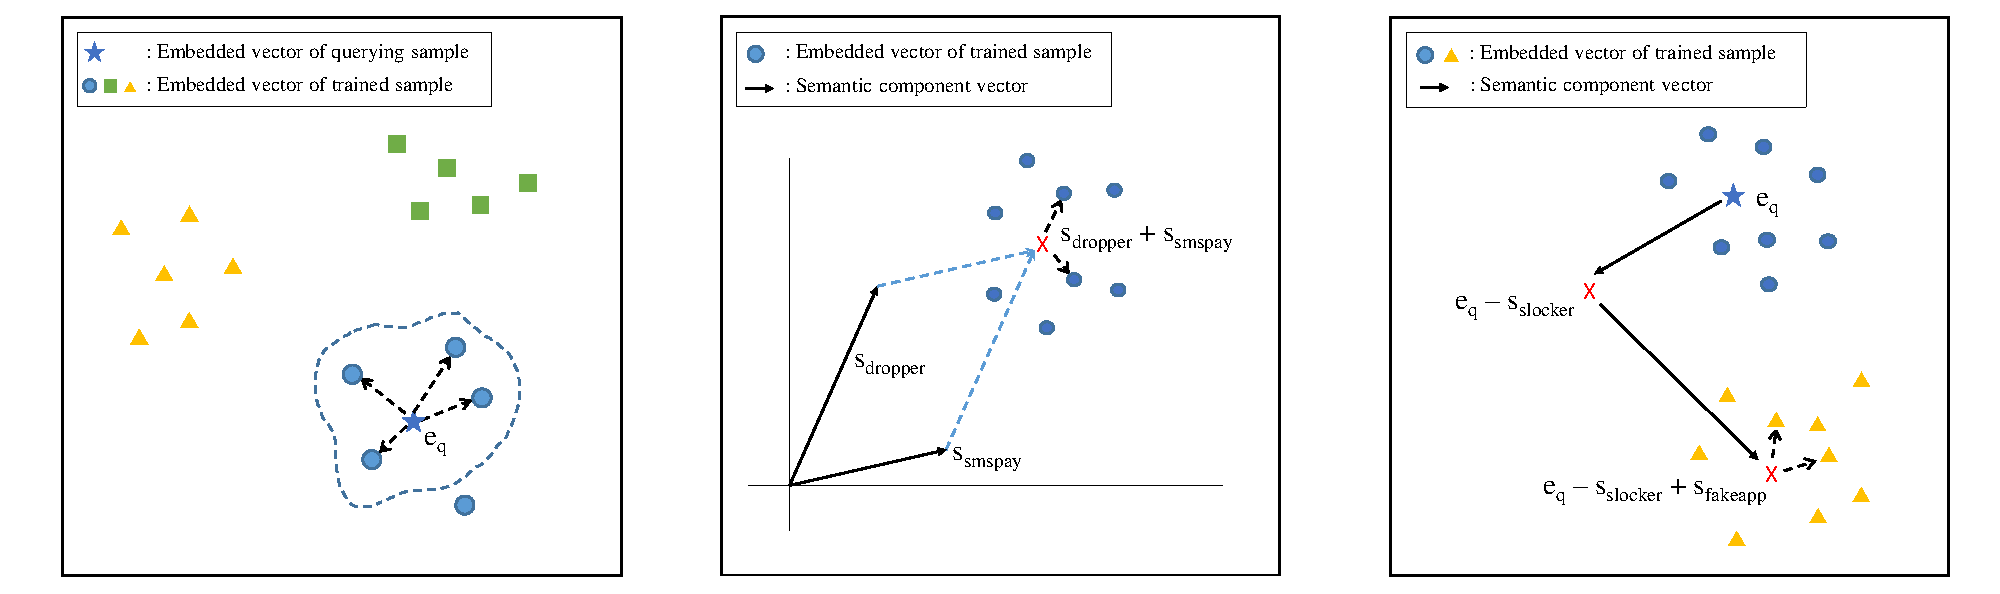
\includegraphics[width=\textwidth]{../../figures/qualitative_all_fix.pdf}
  \caption{Queryings}
  \label{fig:qualitative_all}
\end{figure*}

\textbf{Multilabel Classification. }
멀웨어 샘플의 의미를 반영하는 Vector representation E 를 학습시키기 위해 멀티레이블 분류 학습을 Auxiliary Task 로 선택하였다. 이 분류 태스크를 학습하기 위해 뉴럴 임베더 h는 표현 벡터들을 선형 분류기가 분류할 수 있도록 위치시킨다. 기존 대부분의 멀웨어 분류기를 학습하는 연구들은 하나의 레이블로 분류하도록 분류기를 학습한다. 

하지만 멀웨어 도메인에서 하나의 레이블을 특정하고 이를 기준으로 가르치는 Auxiliary Task로 Malware IR System 을 만든다면, 학습하는 임베딩 벡터가 그 샘플의 의미를 담기에 부족한 점이 있다. 첫 째, 멀웨어에 레이블링을 하는 프로세스가 멀웨어의 의미를 표현하는데에 합리적이지 못하다. 멀웨어는 여러 악성 행위들을 동시에 하는 경우가 많다. 하지만 멀웨어를 대분류, 중분류, 소분류 등 하이러키컬한 분류 체계를 갖도록 레이블링 하는 경우가 대부분이다. 또한 네이밍 규칙이 글로벌하게 일관되지 못하고 심지어 로컬하게도 분석가들 마다 다른 기준으로 네이밍을 하는 경우가 많다. 유행하는 멀웨어에 대해서는 그 멀웨의 레이블을 붙일 때 그 멀웨어의 행위와 상관 없는 특징을 이름으로 붙이기도 한다. 이러한 레이블링 프로세스들은 머신러닝 모델이 멀웨어를 입력으로 받아서 레이블을 예측하는 Supervised Learning Task 를 수행할 때 멀웨어의 의미를 배우는 것을 방해한다. 

둘 째는 하나의 레이블이 만약 Trojan이나 Adware 같은 대분류라면 같은 분류 안의 샘플들을 좀 더 세세하게 구분하여 information retrieval task 를 수행할 때에 정확하게 같은 의미의 샘플을 검색하기가 쉽지 않다. 샘플들의 벡터의 차이가 정확하게 어떤 의미인지를 알 수 없기 때문이다. 레이블이 만약 소분류라면 거의 동일한 샘플들만 같은 분류 안에 속해있을 가능성이 높고, 분류의 개수가 너무 많기 딥러닝 모델의 캐퍼시티가 충분하다면 샘플들을 외우고 하이러키컬 representation 을 학습하지 않아 Generalization 효과가 떨어지게 될 것이다. 따라서 정확하게 같은 샘플들 혹은 아주 약한 변종들이 검색될 수 있지만 의미가 비슷한, 동일하지 않은 샘플들에 대해서는 검색되지 않을 가능성이 높다. 

우리는 같은 의미를 가진 스트럭쳐가 다른 샘플들 뿐만 아니라 비슷한 의미를 가진 멀웨어 샘플들에 대해서도 Retrieval이 가능하도록 하기 위해, 멀티 레이블을 분류하도록 Auxiliary Task 를 학습시키고, 거기에서 얻은 Vector representation 을 검색 시스템에서 사용한다. 이는 여러 의미 계층에 대한 공통 피쳐를 딥러닝 모델이 모두 학습할 수 있도록 도와준다. 


\textbf{Centerloss. }
위의 방식대로 Multilabel Classification 을 학습시키면서 임베딩한 멀웨어의 Representation vector 들이 우리가 정의한 Semantic Space 위에 존재하도록 하려면 SingleLabel 센터로스를 발전시켜 만든 Multilabel Centerloss(MCL) 를 사용해야 한다. 
The first reason is about the variance of samples in the same class. 일단 기존 센터로스의 효과는 인트라 클래스의 베리언스를 낮춰주는 것이라고 백그라운드에서 설명했다. 약간 더 부연 설명을 하자면, 센터로스를 사용하면 inner class variance 가 너무 커서 ranking module 에서 같은 클래스 내 두 샘플의 거리가 서로 다른 클래스 내의 두 샘플 간 거리보다 더 커지는 현상을 막아주어 결과적으로 IR 결과를 향상시킨다. 

두 번째 이유는 우리가 정의한 시멘틱 스페이스의 성질을 만족시키도록 멀웨어 representation vector 를 임베딩 시킬 수 있다는 것이다. 싱글레이블 센터로스를 제안했던 논문에서는 각 레이블 별로 템플릿 벡터를 익스터널 메모리에 저장해놓고 그 템플릿 벡터와 보틀넥의 거리가 작아지도록 MSE 에러를 설정한다. 이는 곧 템플릿 벡터의 속성을 정의하지는 않았지만, 특정 클래스에 해당하는 샘플의 보틀넥은 그 클래스에 해당하는 템플릿 벡터가 되도록 가르칠 수 있다는 것을 의미하고 이 부분이 우리가 센터로스를 사용하여 우리의 문제를 해결해야겠다고 영감받은 부분이다. 마찬가지로 각 시멘틱 컴포넌트 별로 벡터를 익스터널 메모리에 저장해놓고, 보틀넥이 시멘틱 컴포넌트 벡터들의 linear combination 이 되도록 MSE 에러를 로스펑션으로 설정했다. 이 로스에 의해서 우리는 멀웨어의 시멘틱스 벡터가 시멘틱 컴포넌트의 리니어 컴비내이션으로 만들어지는 것을 학습시킬 수 있다. 

%그리고, 보틀넥과 시멘틱 컴포넌트들의 합의 차이에 alpha/the number of answer labels 만큼의 곱을 하여 각 레이블을 업데이트해준다. 알파는 하이퍼파라미터로, 템플릿 벡터와 보틀넥을 얼마나 섞어서 기존 템플릿벡터를 업데이트할지를 결정해주는 값이다. 

\textbf{Learn to Rank. }
멀웨어의 레이블 중에는 우리가 중요하게 여기는 레이블들과 아닌 레이블들이 있다. 멀웨어 retrieval 시스템을 만들 때 이 중요도를 고려하는 것은 semantic understanding property 를 만족시키기 위한 중요한 요소 중 하나이다. 예를 들어 PE 포멧의 레이블들 중, agent 나 downloader보다 ransom, coinminer 등의 레이블에 더 가중치를 주어서 랭킹을 한다면 더 semantics-aware 한 검색 시스템이라고 여길 수 있을 것이다. 이렇게 어떤 시멘틱 컴포넌트에 대해서 더 잘 검색되게 할 지를 IR 시스템을 만들 때 반영하기 위해, 우리는 태그들의 중요도를 constraint 로 추가한 Centerloss 를 사용한다. 여기에서 Constraint 는 시멘틱 컴포넌트들의 Norm을 결정짓는다. 우리가 리트리벌에서 사용하는 Metric function 인 유클리디언 디스턴스는 거리를 계산할 때 두 벡터의 Norm 에 영향을 받는다. Norm 이 큰 semantic component vector 와 다른 컴포넌트 벡터와의 거리는 Norm 크지 않은 컴포넌트 벡터들간의 거리보다 더 크게 될 가능성이 높다. 따라서 euclidean distance 로 랭킹을 하는 IR 시스템에서는 중요도가 큰 semantic component 를 갖고있는 멀웨어를 검색했을 때, 해당 semantic component 를 포함하는 멀웨어 샘플들이 검색될 가능성이 더 높아지게 된다. 이는 기존 IR 시스템에서 특정 속성을 가진 문서들이 더 잘 검색되게 만드는 Scoring 기법 (ex. tf-idf) 과 같은 역할을 하는 것이라고 볼 수 있다. 

%원래 리트리벌에서 랭킹을 위한 스코어링은 원래 하는짓인데 이걸 딥러닝에서 되게 한건 노블한거다. 연역적으로 왜 이렇게 해야하는지는 자명하다.


%\textbf{Semantic space }
%뭘 검색할 수 있어야 우리가 앞에서 문제라고 했던 애들이 해결된다. 연산한걸 검색할 수 있고,...




\subsection{Proposed Objective Functions}
Overview 에서 설명했던 방법들로 말미암아 시멘틱 스페이스를 배우기 위한 새로운 objective function 을 제안한다.  

\textbf{Multilabel Center Loss(MCL). }
우리가 풀고자 하는 constained optimization problem 의 식은 Eq.\ref{eqn:optimization}와 같다. 이는 cross-entropy loss의 근간이 되는 Negative Log Likelihood function 최적화 문제에 target semantic vector 와 representation vector 의 거리가 $\epsilon$ 미만이어야 한다는 constraint 를 추가한 것이다. 

\begin{equation}
\label{eqn:optimization}
\min_{\theta, w, b} J(\theta, w, b) = -\sum_i{ \sum_j{ y_{mij} \log{\hat{y_{ij}}}}}
\end{equation}

s.t.
\[
h(v_i;\theta)) - \mathbf{s}_\text{target} < \epsilon ,
\]
%\[
%||c_i||_2 = cc_i
%\]
for $i \in \{1,2, ..., N\}$ where $\epsilon >= 0$ and $s_\text{target}$ is a target semantic vetcor.

위의 식을 만족시키는 parameters 를 찾기 위해 cross-entropy loss 와 multilabel centerloss 를 1: lambda 의 비율로 더해서 최종 loss function 을 만들었다\cite{}. 우리가 제안하는 loss function 을 수식으로는 Eq.\ref{eqn:centerloss}과 같이 formulate할 수 있다. 

\begin{equation}
\label{eqn:centerloss}
\begin{aligned}
L &= L_s + \lambda L_c \\
 &= -\frac{1}{N}\sum_i{\sum_j{ y_{mij} \log{\hat{y_{ij}}}}} 
+ \lambda \frac{1}{N} \sum_i{( \mathbf{s}_{\text{target}} - h(v_i;\theta))^2}\\
\end{aligned}
\end{equation}

where 
\[
\hat{y_{ij}} = \frac{exp(Wh(v_i;\theta)+\mathbf{b})}{ 1 + exp(Wh(v_i;\theta)+\mathbf{b})}
\]

%$L_c = \sum_i^N{||e_i - s_\text{target}||^2}$

  
\textbf{Weighted Multilabel Center Loss(WMCL). }
앞서 설명한 것 처럼 우리의 Malware Information Retrieval System 에 Learn to rank 기법을 적용시키기 위해 Importance coefficients 를 각 시멘틱 컴포넌트 별로 부여한다. 기존 Multilabel Center Loss 에 semantic component vector 의 norm 과 importance coefficient 값이 같도록 하는 constraint 를 하나 더 추가하여 중요도를 반영하였다.
\[
||s_i|| = c_i \text{ for all i }\in \{i = 1,2, ..., M\}
\]


cross-entropy 로스는 multilabel classification 의 accuracy 를 높이기 위해 $\theta, W, \mathbf{b}$의 파라미터들을 업데이트시킨다. multilabel centerloss 을 통해 업데이트하는 대상은 크게 두 가지가 있다. 하나는 embedding vector 가 $\mathbf{s}_{\text{target}}$ 와 가까워지도록 $\theta, W, \mathbf{b}$ 의 parameter들을 back propagation 을 통해 업데이트시킨다. 두 번째는 $\mathbf{s}_{\text{target}}$가 embedding vector 와 가까워지도록 semantic compoenents 를 업데이트시킨다. 업데이트 할 때는 다음 step 에서의  $\mathbf{s}_{\text{target}}$ 가 지금의 $\mathbf{s}_{\text{target}}$ 와 임베딩 벡터의 $\alpha$: $1-\alpha$ 내분점이 되도록, 두 벡터의 difference vector를 각 semantic compoenent vector 에게 균등하게 나눠 더해주어 업데이트 한다. 
semantic component vectors 를 더해서 target semantic vector 를 만드는 모델(summation model) 과 평균으로 만드는 모델(average model) 이 있다. 각 모델의 성능은 Section 5. 에서 확인할 수 있다. 

파라미터와 semantic component update 의 과정은 Figure.\ref{fig:update} 와 Algorithm.\ref{alg:centerloss} 그리고 Algorithm.\ref{func:functions}에서 확인할 수 있다. 

%average model 은 semantic component 가 추가되거나 제거될 때 embedding vector 의 변화가 많이 필요하지 않다는 장점이 있다. 어떤 semantic component 를 갖고 있는지 모르는 Sample 과 semantic component 의 조합으로 쿼링하는 태스크를 수행하기 어렵다는 단점이 있다. 

%\textbf{Statistical view. }

\begin{figure}[!htb] % update
  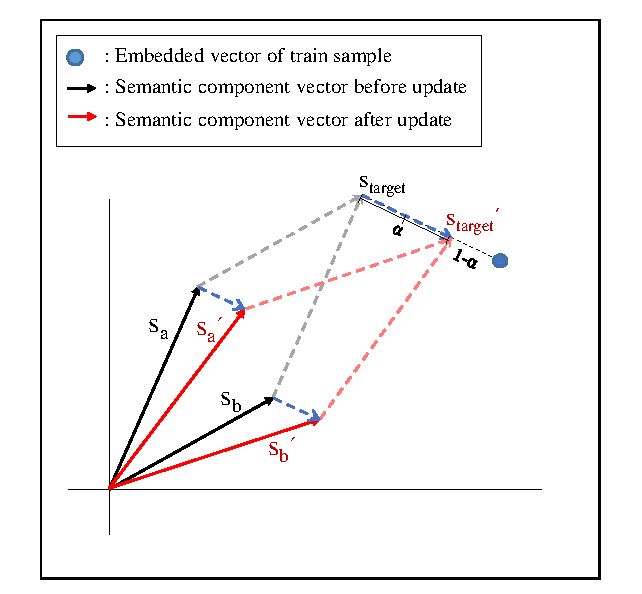
\includegraphics[width=\columnwidth]{../../figures/update.pdf}
  \caption{update}
  \label{fig:update}
\end{figure}



\begin{algorithm}[!htb]%centerloss
\SetAlgoNoLine
\SetKwFunction{Ftarget}{getTargetSemanticVectors}
\SetKwFunction{Fnew}{getNewSemanticComponentVectors}

\KwIn{Extracted handcrafted features of training data $v_i$ and their semantic components $\mathbf{y}_i$. Initialized parameters $\theta$ in neural embedder. parameters $W, b$ in classifier. initialized semantic component vectors $\mathbf{s}$.Importance coefficients $\textbf{c}$. Hyperparameter $\lambda$, $\alpha$, learning rate $\mu$. }
\KwOut{The parameters $\theta$, $W$, $b$ }
\Repeat{converge}{
    $s_\text{target} = \Ftarget(s_{\mathbf{y}})$ \\
	Compute total loss by $L = L_s + \lambda L_c$\\
	Update parameters $\theta$ by $\theta \leftarrow \theta - \mu \frac{\partial L}{\partial\theta}$ \\
	Update parameters $W$ by $W \leftarrow W - \mu \frac{\partial L}{\partial W}$\\
	Update parameters $b$ by $b \leftarrow b - \mu \frac{\partial L}{\partial b}$\\	
	Update semantic component vectors $s$ by $s \leftarrow \Fnew()$
	

	}
	\caption{The semantics-aware representation vector learning algorithm. }
\label{alg:centerloss}
\end{algorithm}


\begin{algorithm}[!htb]%functions
  \SetAlgoNoLine
  \DontPrintSemicolon
  \SetKwFunction{Ftarget}{getTargetSemanticVectors}
  \SetKwFunction{Fnew}{getNewSemanticComponentVectors}
  
  \SetKwProg{Fn}{Function}{:}{}
  \Fn{\Ftarget{$\mathbf{s}$}}{
    $M \leftarrow $ The number of semantic components \\
  	
    
	\If{Summation Model}
	{$s_{\text{target}} \leftarrow \sum_i^M{s_i}$}
	\ElseIf{Average Model}
	{$s_{\text{target}} \leftarrow \frac{1}{M}\sum_i^M{s_i}$}    
    
    \KwRet $s_{\text{target}}$\;
  }
  \;
    
  \SetKwProg{Pn}{Function}{:}{}
  \Pn{\Fnew{$\mathbf{s}$, $s_{\text{target}}$, $e$, $\alpha$, $\mathbf{c}$}}{
    $M \leftarrow $ The number of semantic components \\
    \ForEach{$i \in \{1, 2, ..., C\}$}{
	  \If{Summation Model}
	  {$s_i \leftarrow s_i - \frac{\alpha}{M}(s_{\text{target}} - e)$}
	  \ElseIf{Average Model}
	  {$s_i \leftarrow s_i - \alpha (s_{\text{target}} - e)$ }
	  \If{Weighted Model}
	  {$s_i \leftarrow \frac{s_i}{||s_i||} c_i$}    
    }
    \KwRet $\mathbf{s}$
  }
  \;  

  \caption{Definitions of functions. }
\label{func:functions}
\end{algorithm}
